\documentclass[11pt]{article}

\usepackage[margin=1in]{geometry}
\usepackage{fancyhdr}
\pagestyle{fancy}
\usepackage{amsmath}
\usepackage{amssymb}
\usepackage{graphicx}
\lhead{Chaitanya Pawa}
\chead{Statistical Data Mining II\ Homework 2}
\rhead{March 1, 2019}


\begin{document}

\begin{enumerate}
\item \textbf{Problem 1}
\\
In this exercise, we consider the USArrests data. The data set consisted of 50 observations with 4 variables. We performed hierarchical clustering on the states.
\begin{enumerate}
    \item We used hierarchical clustering with complete linkage and Euclidean distance to cluster the states.
    \\We received the following dendrogram for the above.
    \begin{center}
    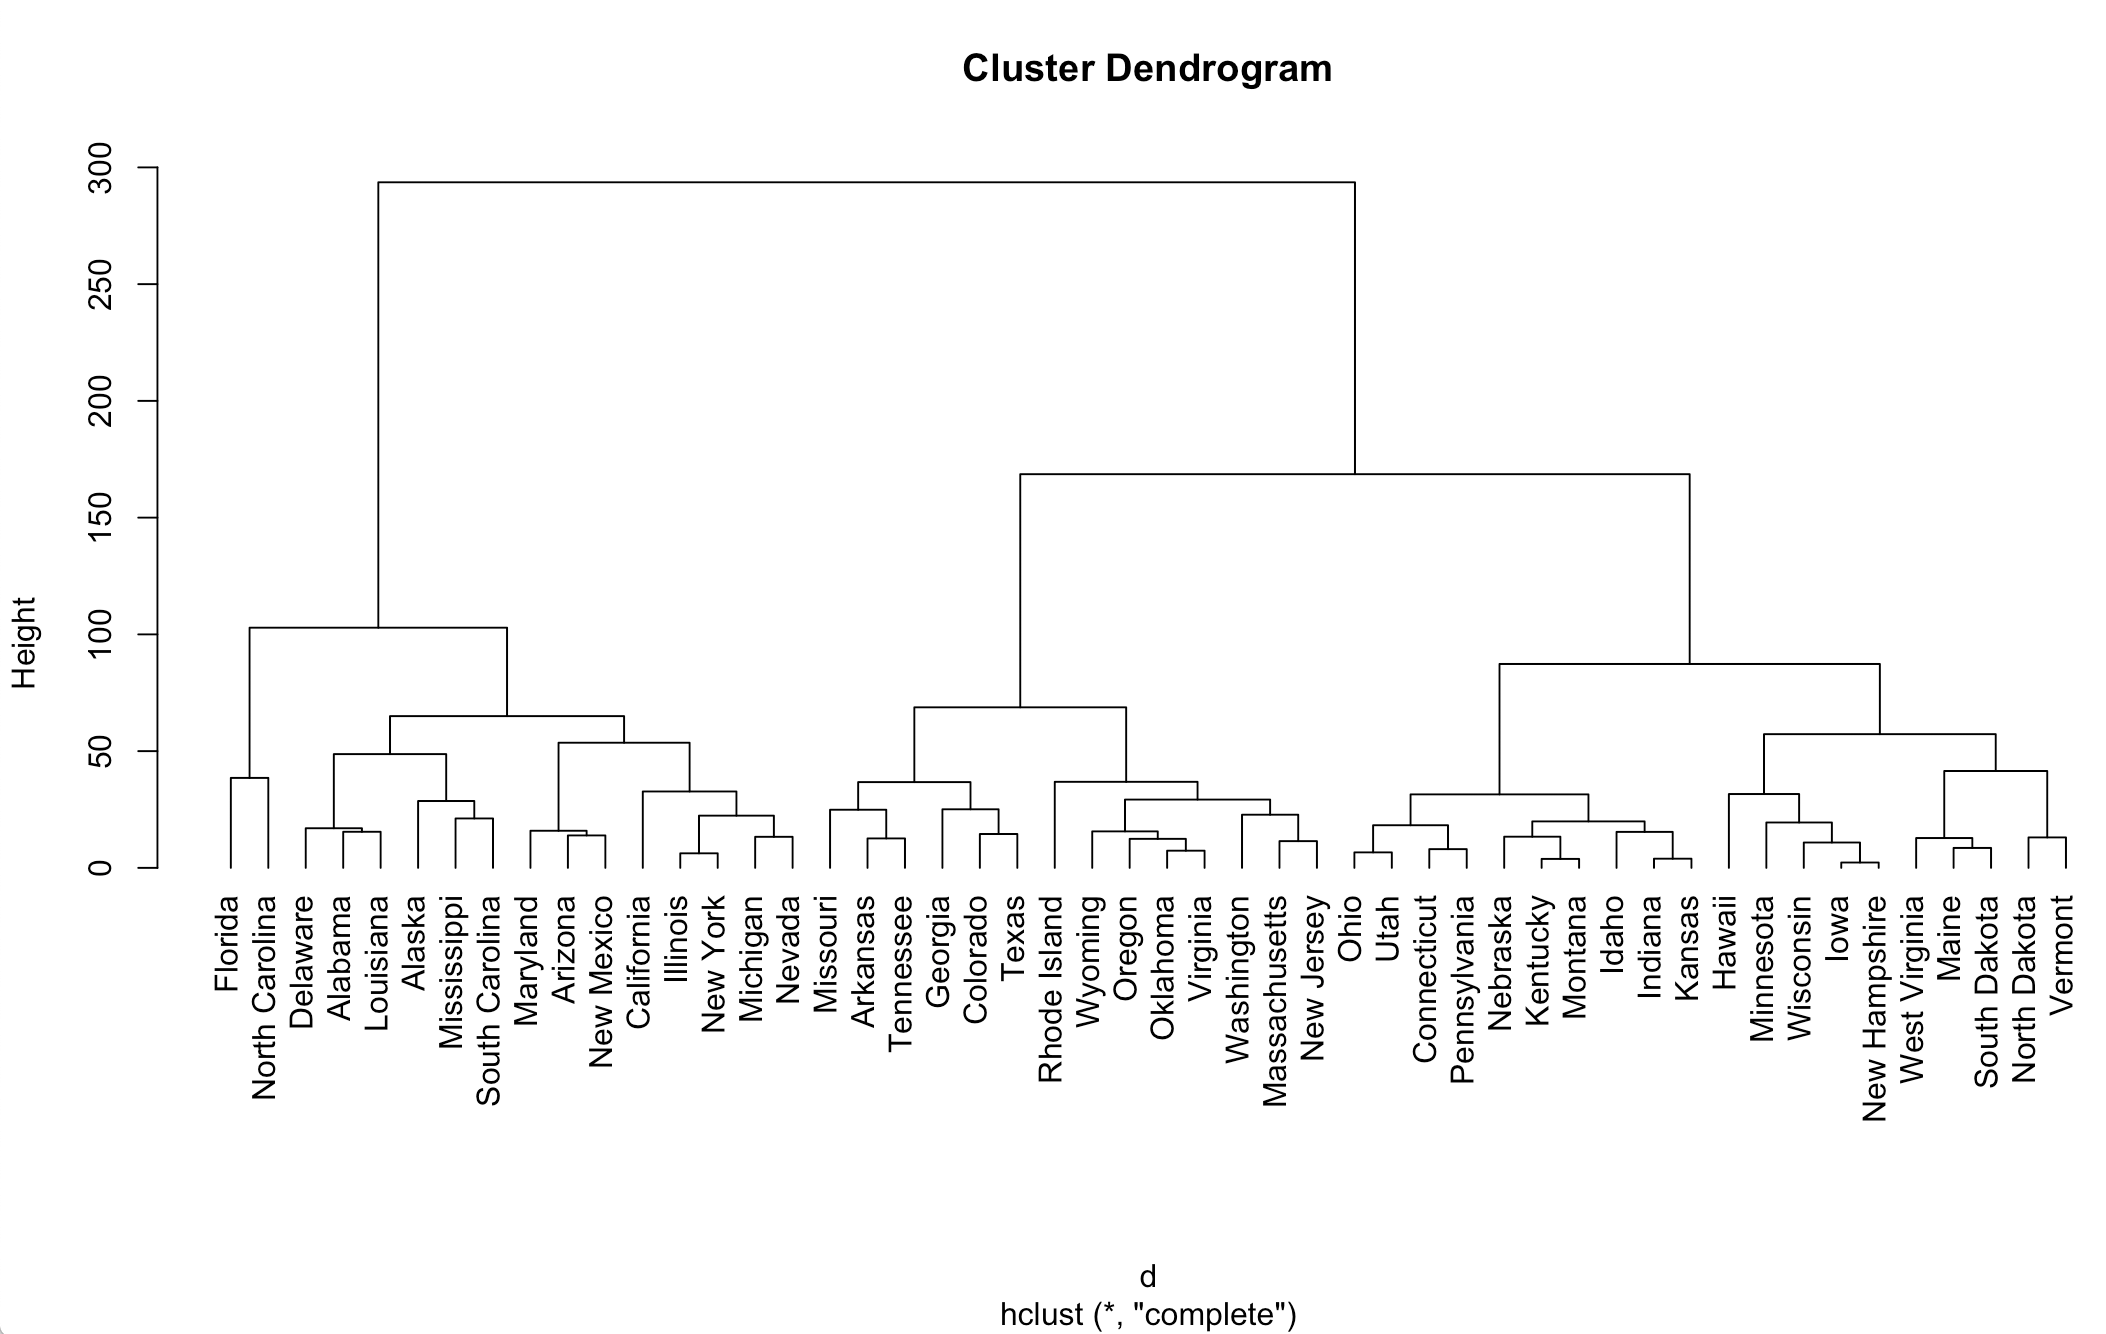
\includegraphics[width=0.8\textwidth]{1_A.png}
    \\\footnotesize Figure 1.1 : Cluster Dendrogram for Complete Linkage Hierarchical Clustering
    \end{center}
    \item We cut the dendrogram at a height of 110 so that it resulted in three distinct clusters. The states were categorized into the clusters in the following way.
    
    \begin{center}
    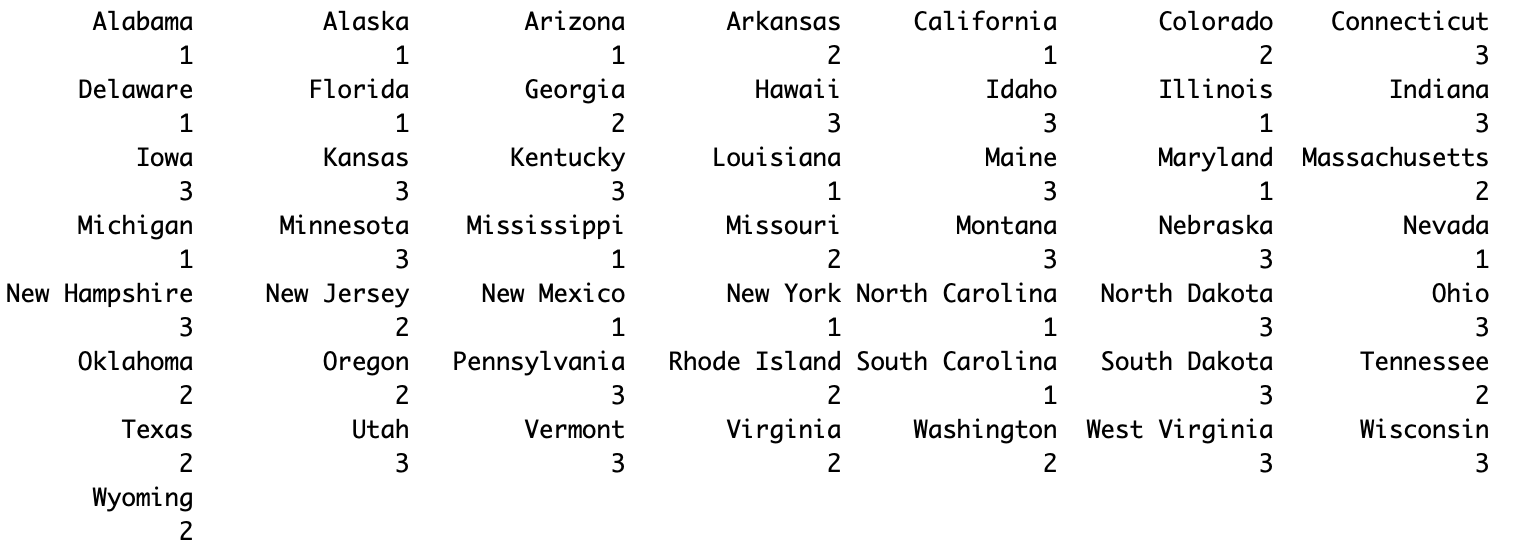
\includegraphics[width=0.8\textwidth]{1_B.png}
    \\\footnotesize Figure 1.2 : Clustering Results
    \end{center}
    
    We also got the following silhouette plot after cutting the dendrogram to get 3 clusters. The clusters had a good values for the average width of the silhouette i.e. 0.53.
    
    \begin{center}
    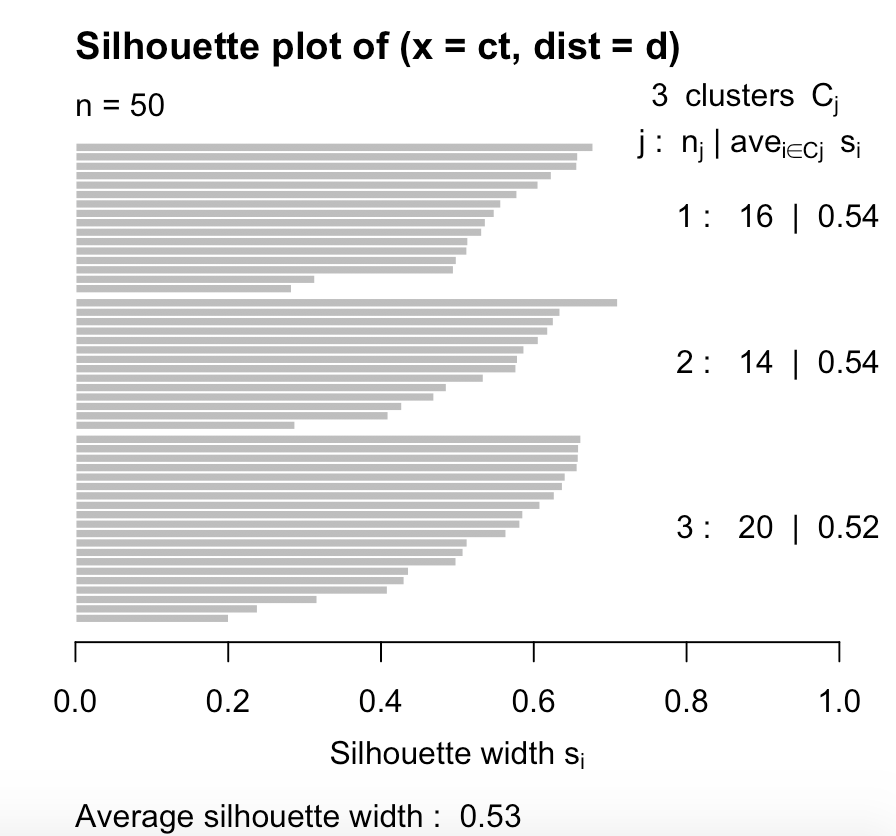
\includegraphics[width=0.5\textwidth]{1_BB.png}
    \\\footnotesize Figure 1.3 : Silhouette Plot
    \end{center}
    
    \item We further scaled the variable to have standard deviation as one and did hierarchical clustering using Euclidean distance and complete linkage. 
    
    \begin{center}
    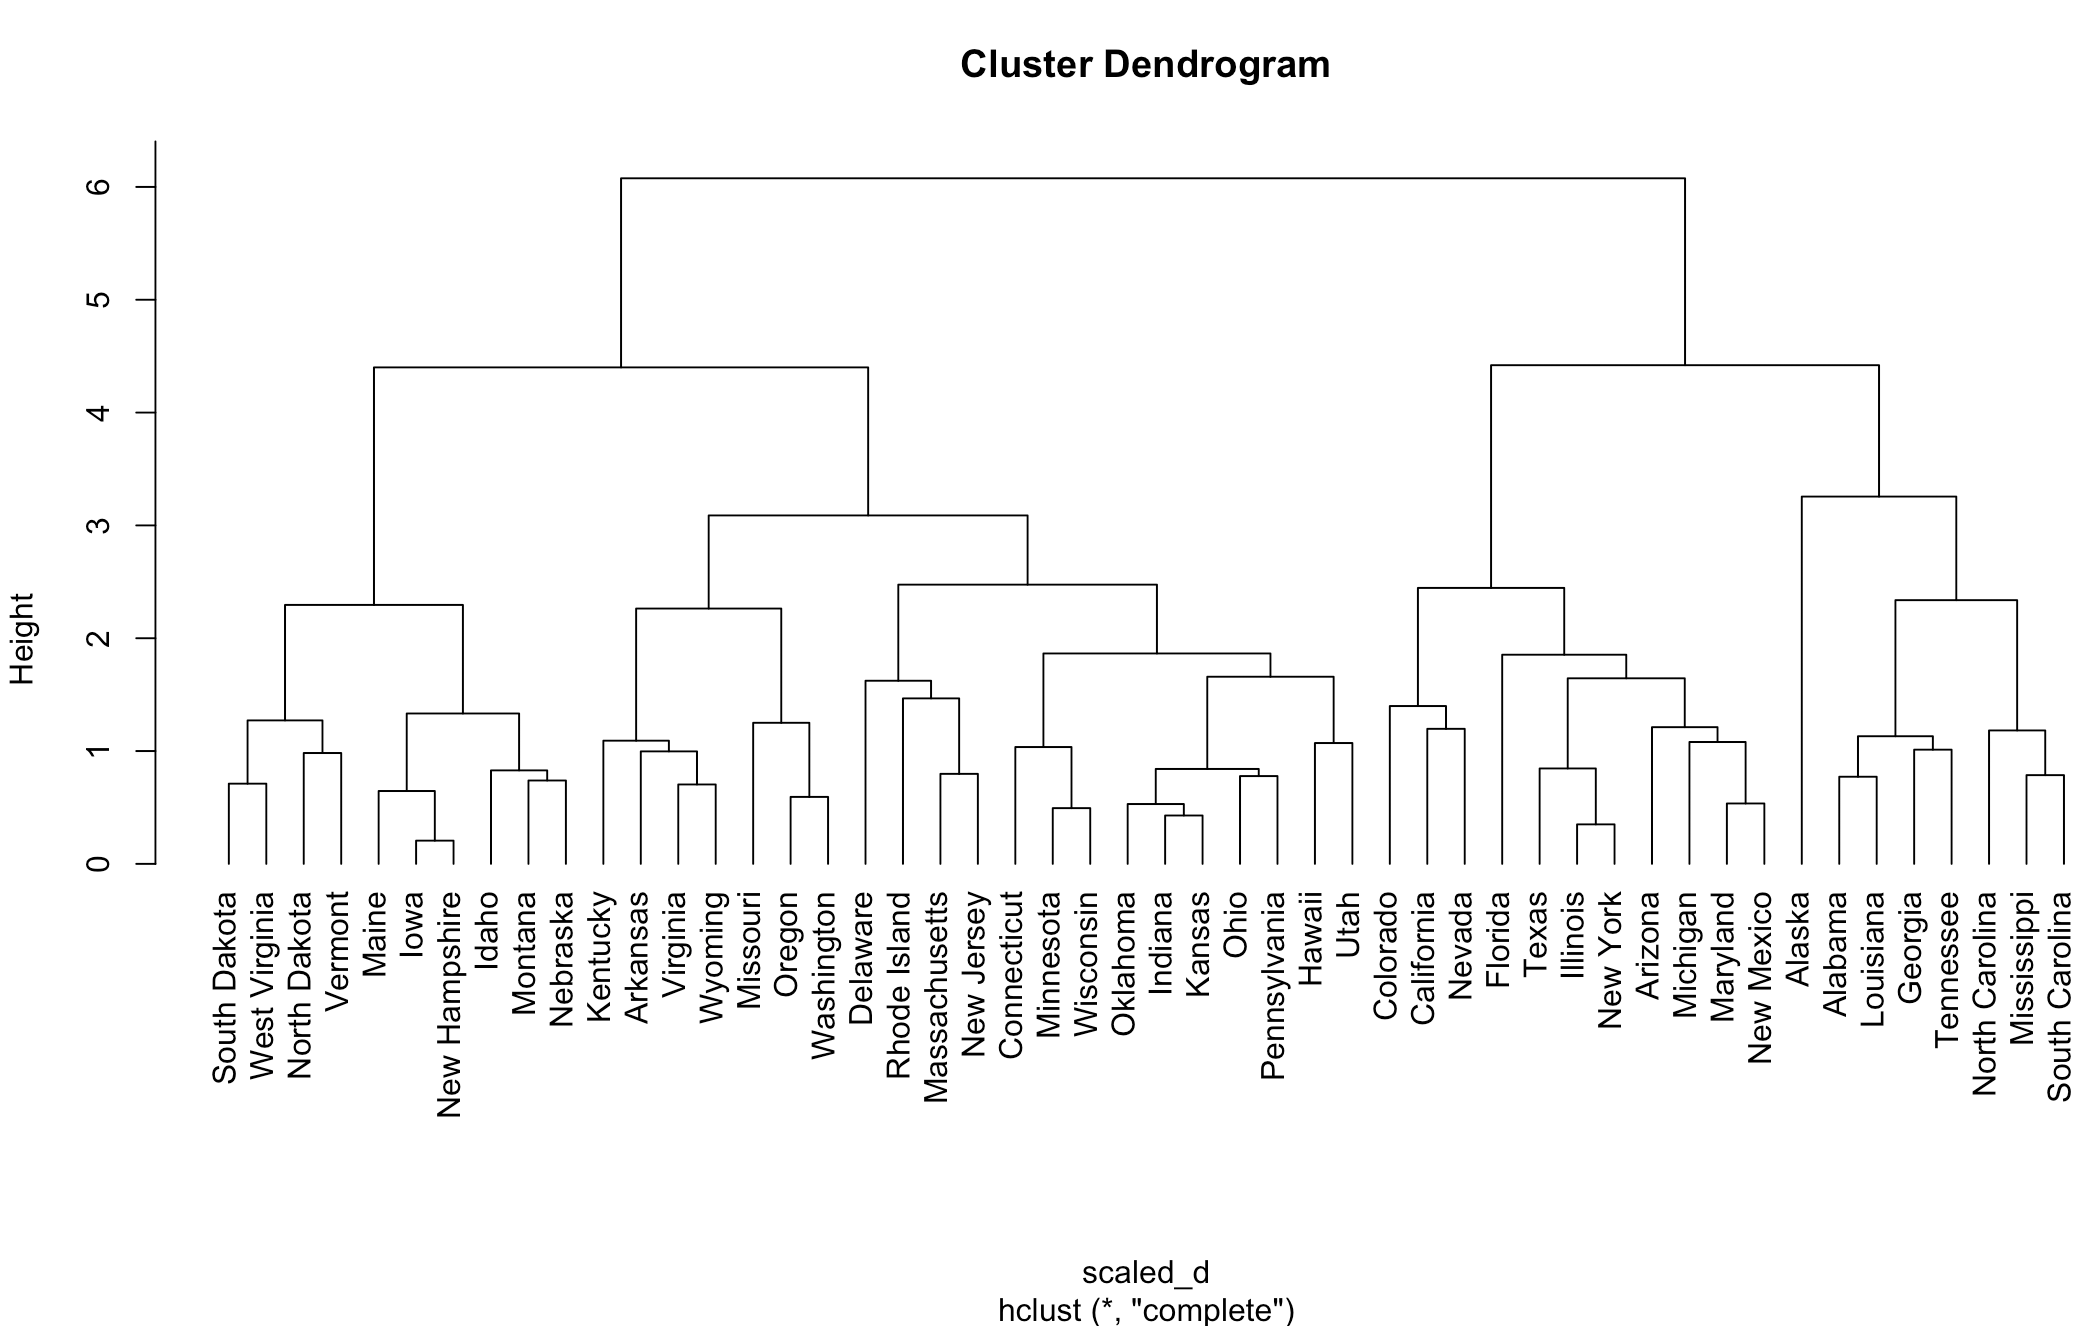
\includegraphics[width=0.8\textwidth]{1_C.png}
    \\\footnotesize Figure 1.4 : Cluster Dendrogram for Complete Linkage Hierarchical Clustering for Scaled Data
    \end{center}
    We got the following silhouette plot after cutting the dendrogram for 3 clusters.
     \begin{center}
    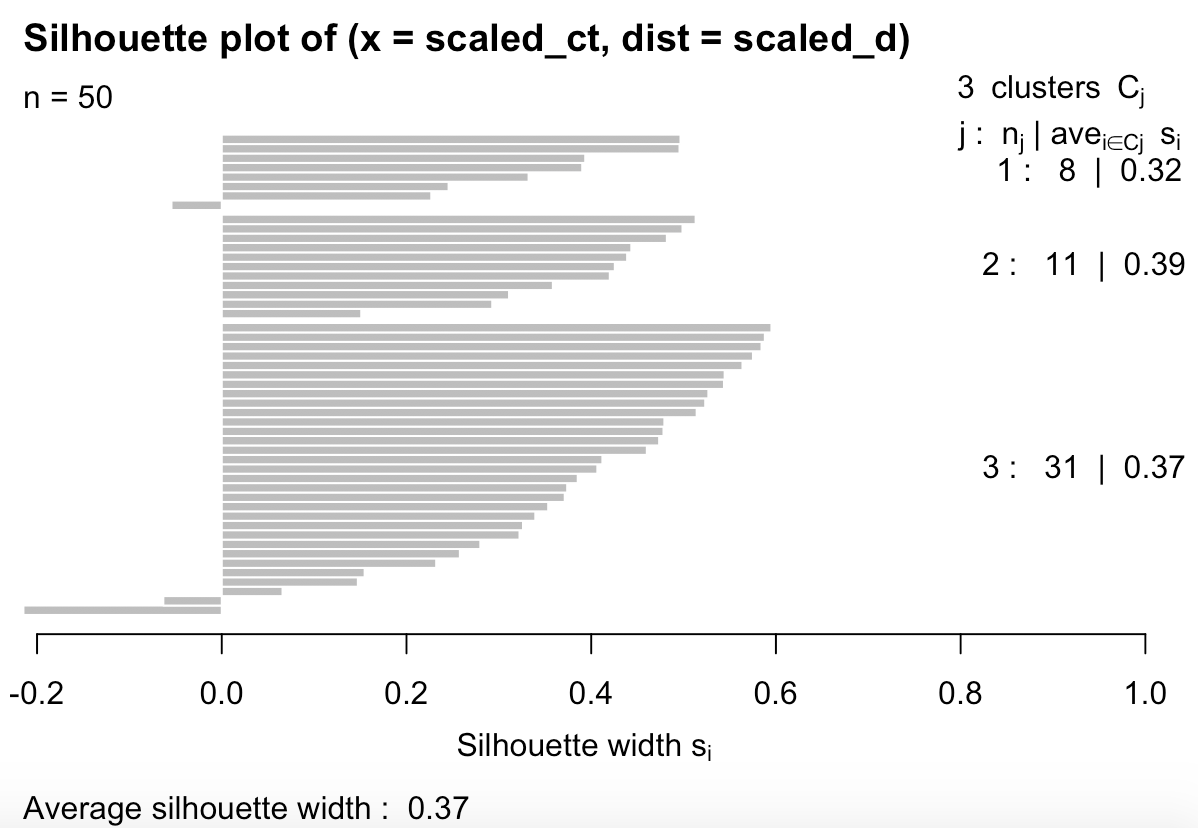
\includegraphics[width=0.5\textwidth]{1_CC.png}
    \\\footnotesize Figure 1.4 : Silhouette Plot
    \end{center}
    
    \item We compared the clustering pre and post scaling  of data using the following table.
    \begin{center}
    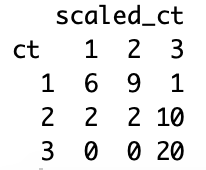
\includegraphics[width=0.2\textwidth]{1_D.png}
    \\\footnotesize Figure 1.5 : Comparison between pre and post scaling
    \end{center}
    
    By scaling the variables, we get lower intra-cluster widths which is better as  for the case of clustering. The more the points are bound to each other, the better will be the clustering model. 
    \\We should scale the variables before the inter-observation dissimilarities are computed because different variables can have different range of values. By having values of the same ranges i.e. by scaling, the clustering models and do a much better job at clustering them accurately.
\end{enumerate}
\newpage
\item \textbf{Problem 2}
\newpage
\item \textbf{Problem 3}
\newpage
\item \textbf{Problem 4}
In this exercise, we ran a batch-SOM analysis on the Wisconsin Breast-Cancer data. 
\\As a part of pre-processing, we removed the first column which contained the id of the observations and separated the true labels from the data to be used for batch-SOM analysis. The data consisted of 357 observations of benign tumor and 212 observations of malignant tumor. 

\\We took a SOM grid of 3X3 dimension with a rectangular topology. We ran the batch analysis by presenting the complete data to the network 2000 times. 

\\We observed the following plots for our batch SOM analysis.

 \begin{center}
    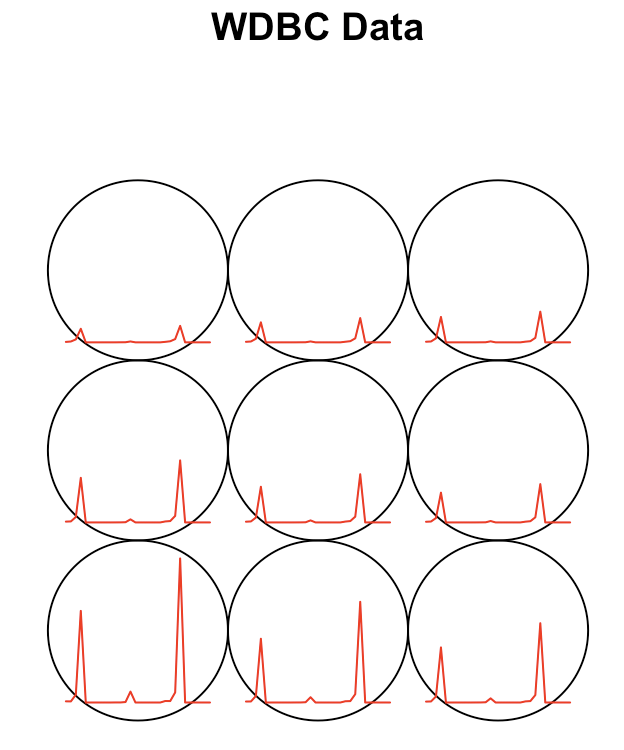
\includegraphics[width=0.4\textwidth]{4_A.png}
    \\\footnotesize Figure 4.1 : WDBC Data
\end{center}
\begin{center}
    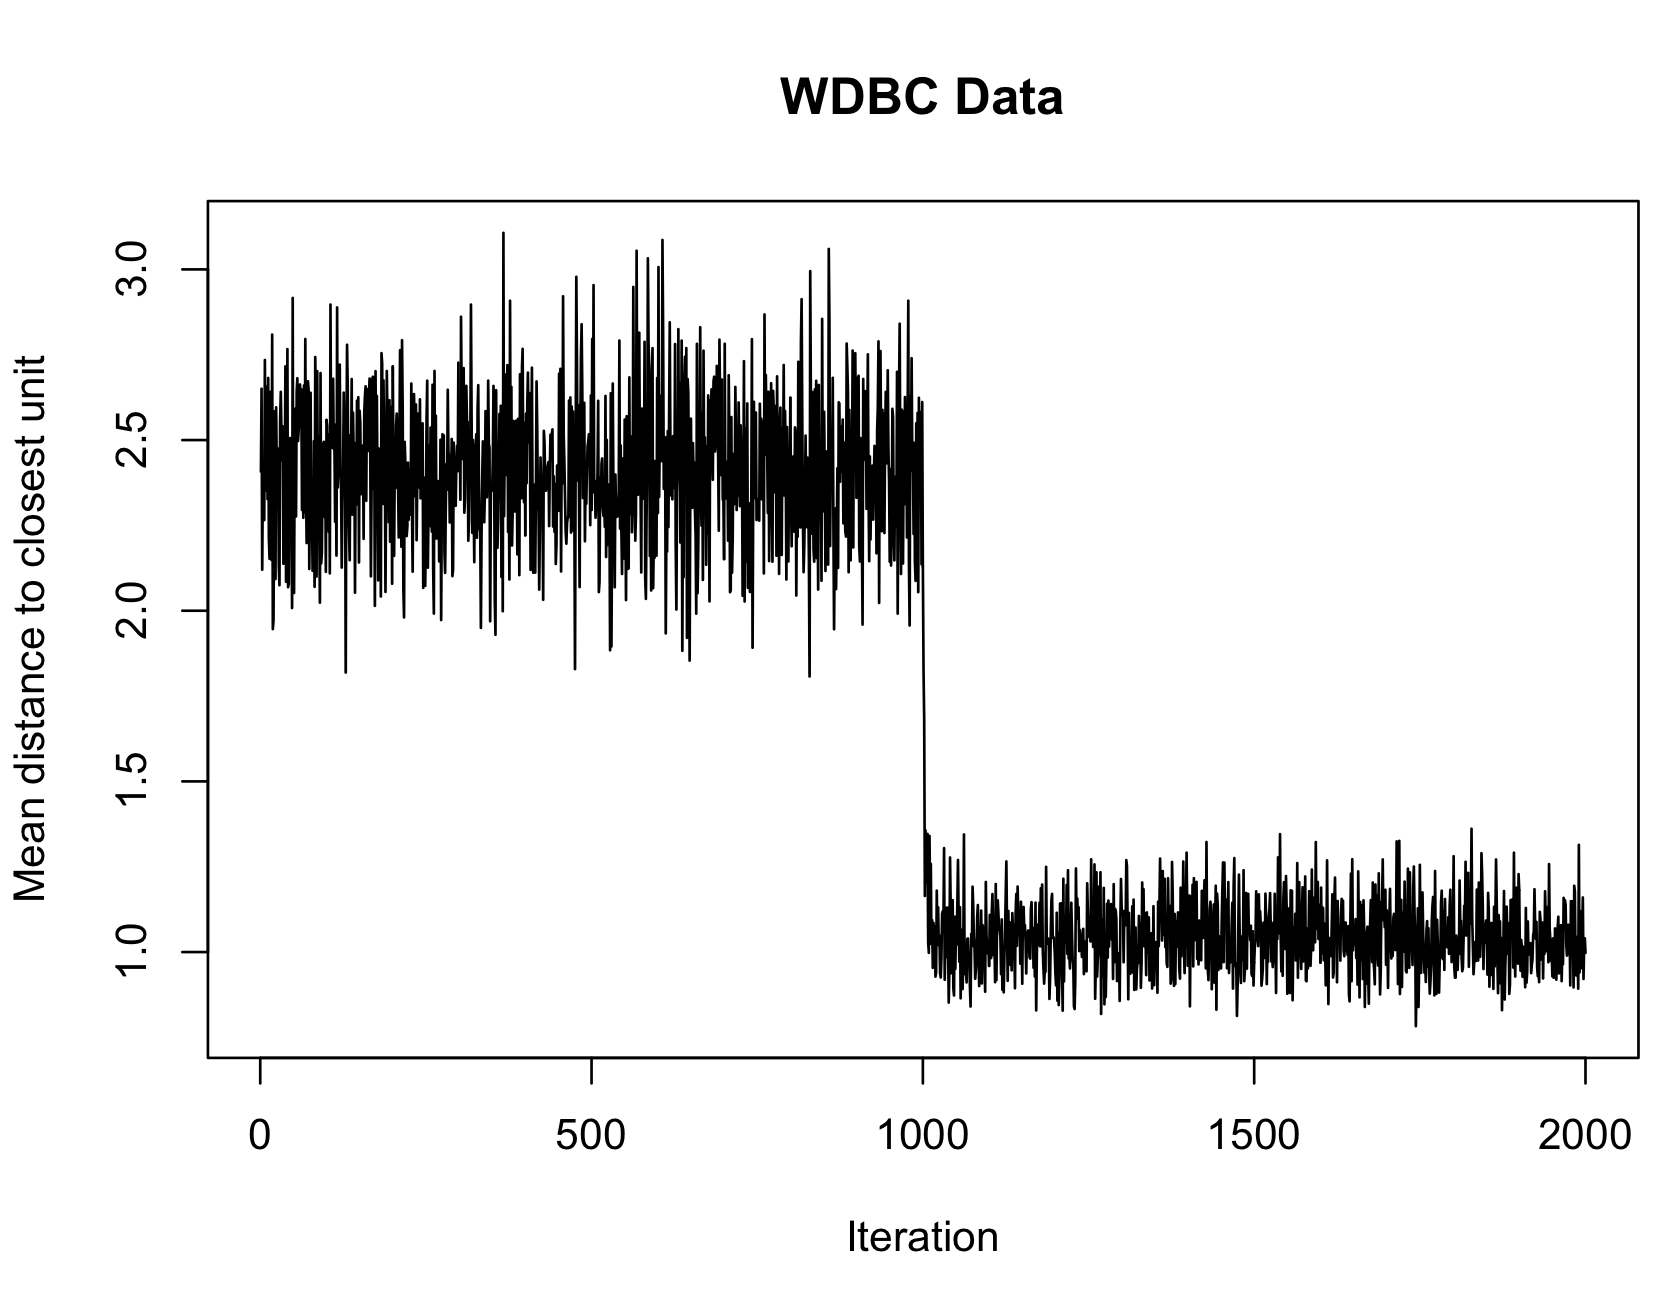
\includegraphics[width=0.4\textwidth]{4_B.png}
    \\\footnotesize Figure 4.2 : Changes in Data
\end{center}
\begin{center}
    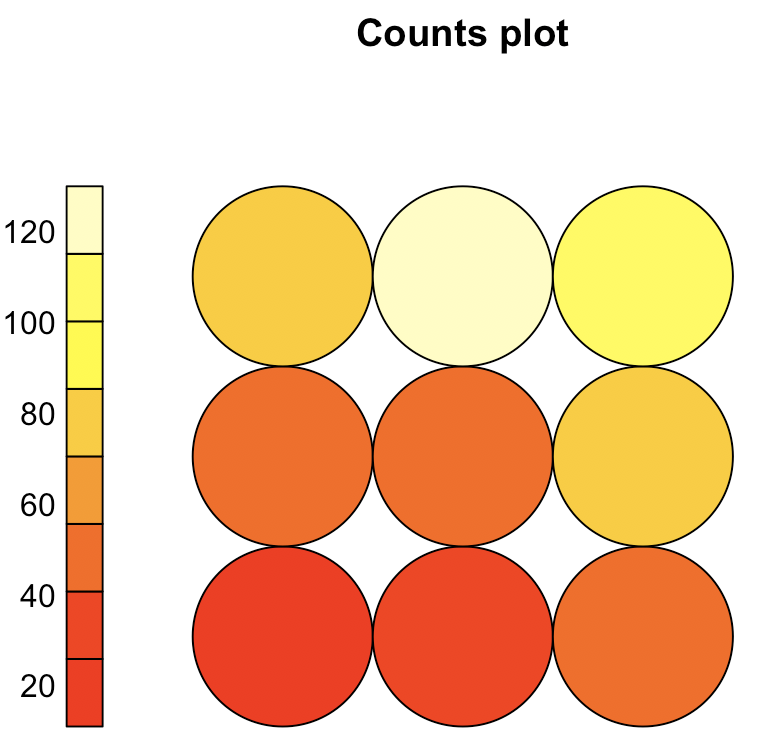
\includegraphics[width=0.4\textwidth]{4_C.png}
    \\\footnotesize Figure 4.3 : Counts Plot
\end{center}
\begin{center}
    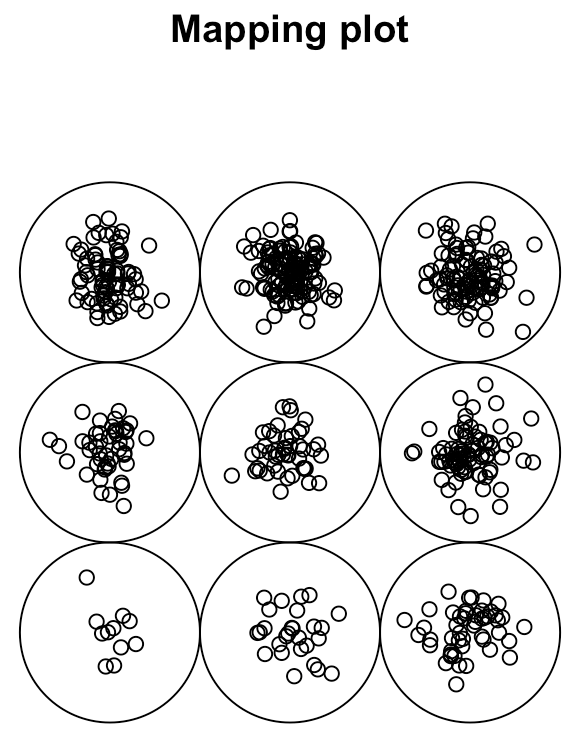
\includegraphics[width=0.3\textwidth]{4_D.png}
    \\\footnotesize Figure 4.4 : Mapping Plot
\end{center}
\begin{center}
    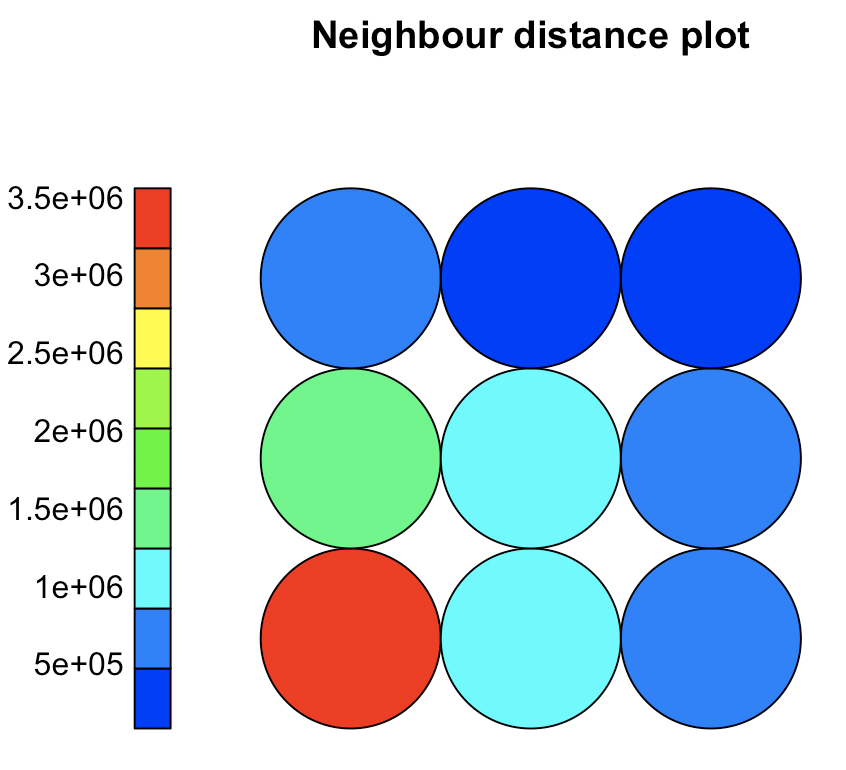
\includegraphics[width=0.4\textwidth]{4_E.png}
    \\\footnotesize Figure 4.5 : Mapping Plot using distance between neighbours
\end{center}

By the above plots, we can see that the batch SOM analysis divided the data pretty well into my 3X3 grid. The counts are well distributed among all the elements of the grid. The mapping of the points are also well distributed apart from one of the elements of the grid. We can also see from the neighbour distance plot that the distance of the neighbours is also what constant.
\\The basic idea behind SOM  batch analysis is to map a  high dimensional data into a lower 2D dimension and we can say from the above plots that the SOM is doing a good job of mapping the observations to 2D.

\\We further carried out  clustering of the data to check for how well the SOM had worked out. The SOM reduced data to be  mapped into 9 categories and we obtained the following dendrogram after clustering the data.

\begin{center}
    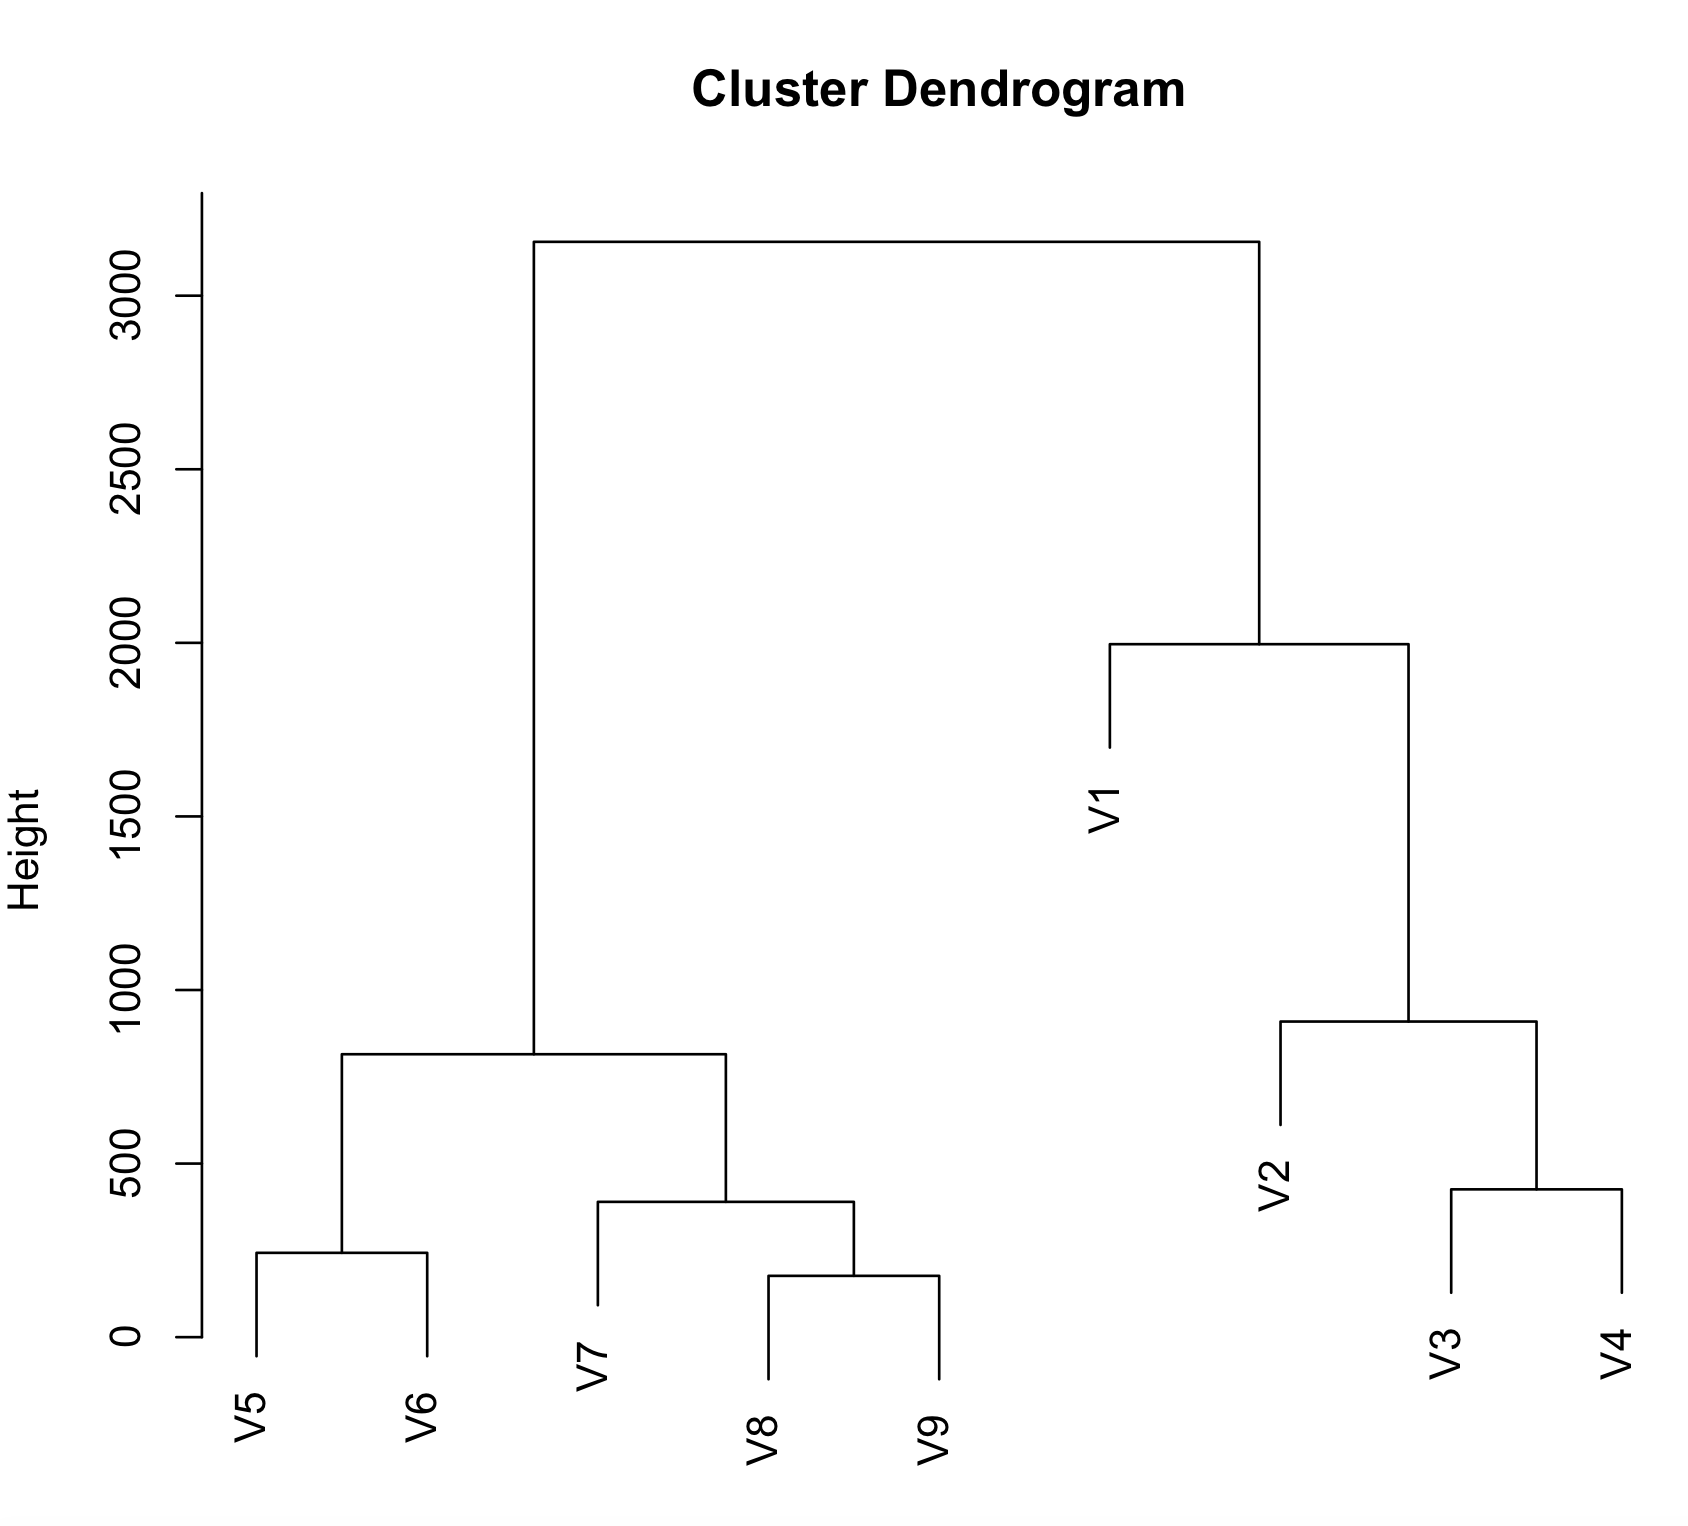
\includegraphics[width=0.5\textwidth]{4_F.png}
    \\\footnotesize Figure 4.6 : Cluster Dendrogram
\end{center}

We further cut the dendrogram into 2 clusters to evaluate the analysis done using SOM by comparing how well it had mapped our clusters. We plotted the SOM with the found clusters.

\begin{center}
    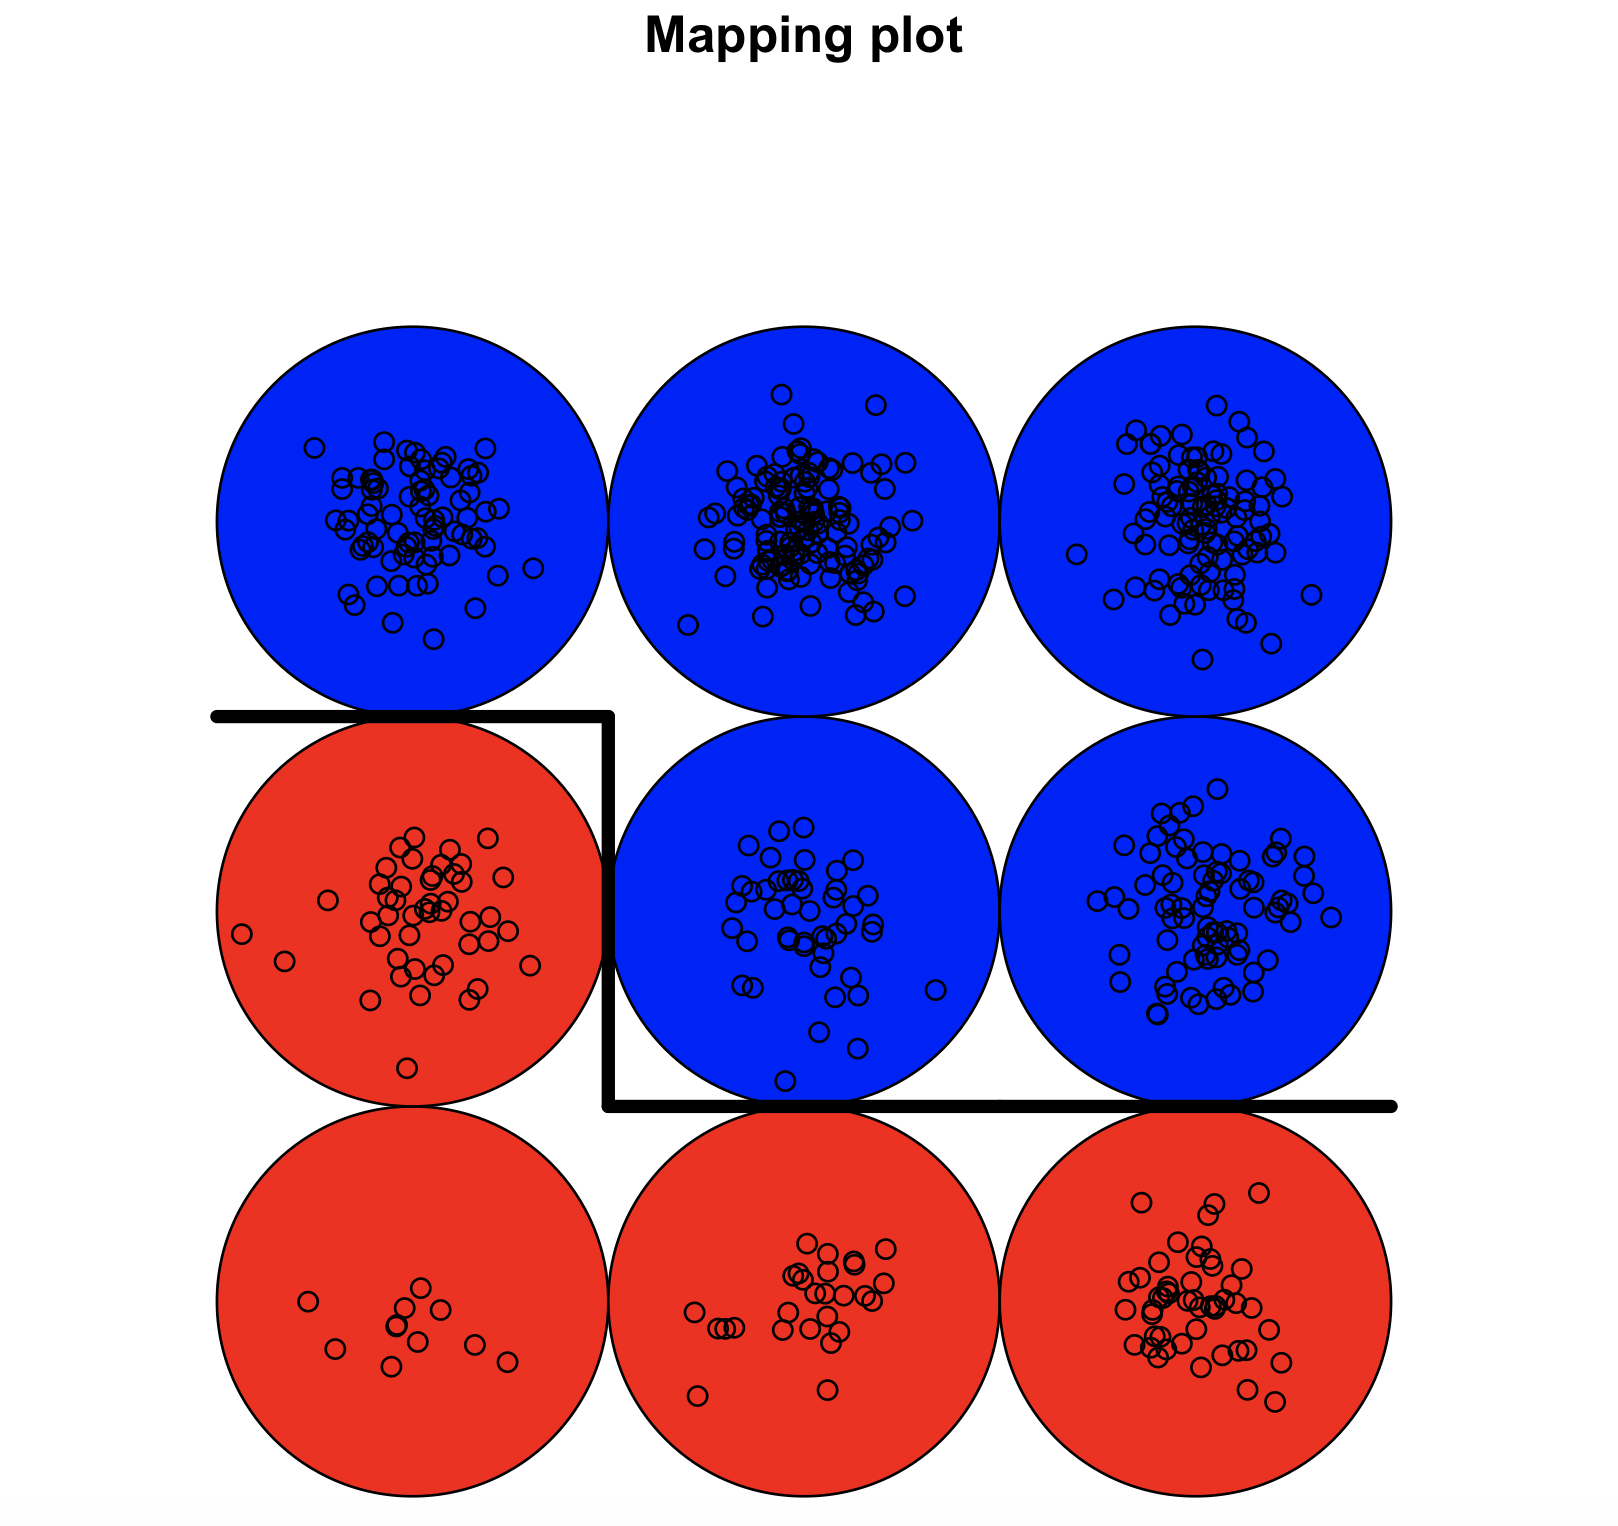
\includegraphics[width=0.5\textwidth]{4_G.png}
    \\\footnotesize Figure 4.6 : Mapping plot of SOM with the clusters
\end{center}

We can see that SOM did a great job in distinguishing between  the benign and malignant tumor. The line segregates the grid elements properly into the two clusters that we received after carrying out hierarchical clustering. Also, the division of data into the two clusters is also somewhat in accordance to my original labels. The misclassification is mostly because of the anomalies in the data or the way it has been clustered. But as for the SOM batch analysis, we can say that it properly divided the two clusters into separate  grid  elements.  



\end{enumerate}
\end{document}